\section{Neural Turing Machines}

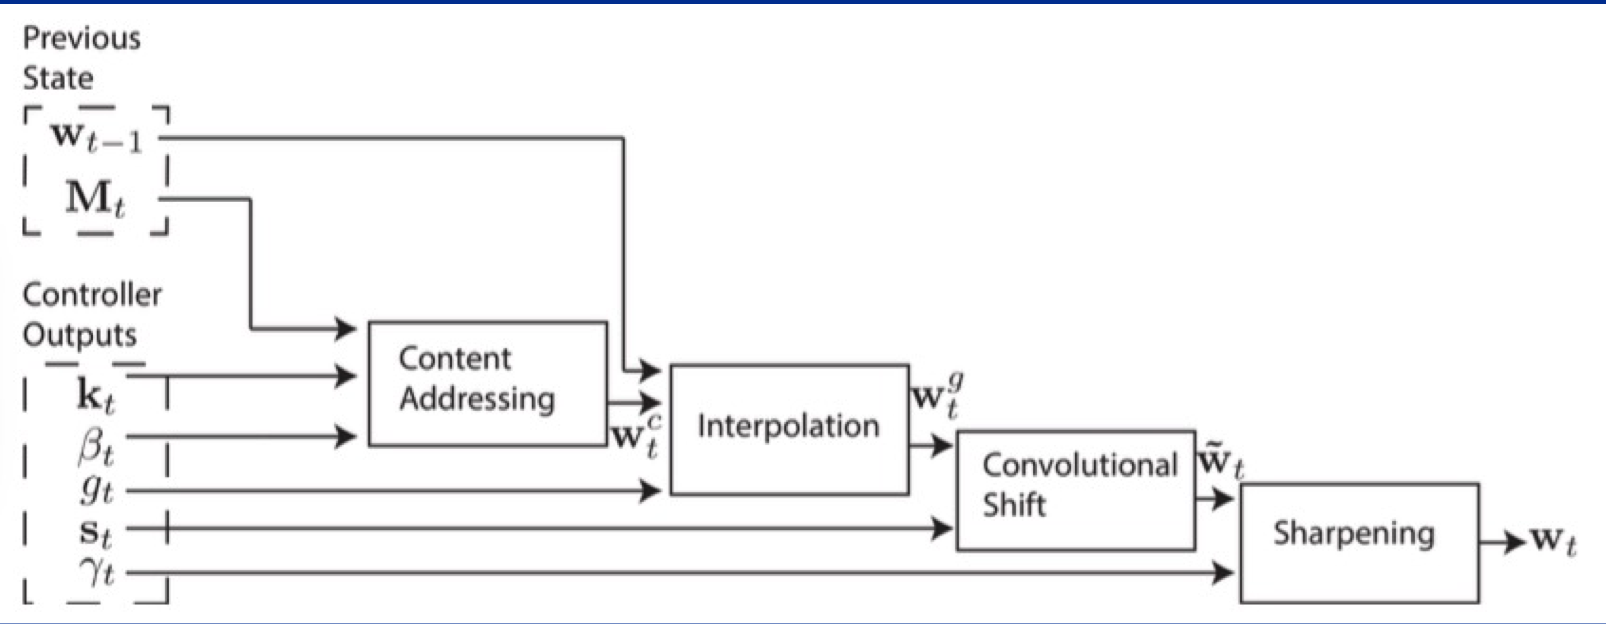
\includegraphics[width=0.9\linewidth]{images/neural_tm}

Can explicitly teach a neural net to program. However, the network must learn how to remember things in its internal state space.

NTMs add structured memory to a neural controller to which it can read/write. \textbf{Controller:} can be feed-forward or recurrent (LSTM units). Recurrent ones typically work better. \textbf{Read} and \textbf{write} heads are content and location addressable. Below $r_t$ is the read vector.

$$ r_t \leftarrow \sum_i w_t(i) M_t(i) $$

$$
M = \begin{bmatrix}
  3 & 1 & 4 & 1 \\
  5 & 9 & 9 & 7 \\
  2 & 7 & 2 & 8 \\
\end{bmatrix}
$$

\[ w = (0, 1, 0)^T, r_t = (5, 9, 9, 7) \]

\[ w = (1/2, 1/2, 0)^T, r_t = (4, 5, 6.5, 4) \]

\textbf{Write} operations happen in two steps: erase then add. Here $e_t$ is the erase vector and $i$ is the location.
$$ M_t(i) \leftarrow M_{t - 1}(i)[1 - w_t(i)e_t]$$

\[ w = (0, 1, 0)^T, e_t = (1, 1, 1, 1) \]

$$
M = \begin{bmatrix}
  3 & 1 & 4 & 1 \\
  0 & 0 & 0 & 0 \\
  2 & 7 & 2 & 8 \\
\end{bmatrix}
$$

Must be done in wo steps because there is no "overwrite" in arithmetic. 

\textbf{Content-based Addressing:} Takes cosine similarity of key vector and memory element. 

\textbf{Location-based Addressing:} Takes location-based addresses and offsets can be used to manipulate specific locations in memory.

NTMs learn to use memory because it is end-to-end differentiable.

NTM with LSTM controller performs best. 
